\documentclass[12pt,slovene]{article}
\usepackage{amsmath,amsfonts}
\usepackage{babel}
\usepackage{comment}
\usepackage{algorithm} 
\usepackage{algpseudocode}
\usepackage{tikz,tikz-3dplot, color}
\oddsidemargin 0in
\textwidth 6.5in
\textheight=9in
\topmargin=-0.5in

\usepackage{mathtools}
\usepackage{url}

\DeclareMathOperator{\LT}{LT}
\DeclareMathOperator{\grad}{grad}
\newcommand{\RR}{\mathbb R}
\newtheorem{theorem}{Izrek}
\newtheorem{definition}{Definicija}
\newtheorem{corollary}[theorem]{Corollary}
\newtheorem{lemma}[theorem]{Lemma}
\newtheorem{proposition}[theorem]{Proposition}
\newtheorem{primer}{Primer}


\begin{document}

\begin{large}\begin{center}
\textbf{Uvod v avtomatsko odvajanje}
\end{center}\end{large}
\bigskip

\section{Uvod}

Učinkovito računanje odvodov je v računalništvu zelo pomembno opravilo. Računanje gradientov funkcij, Hessejevih in Jacobijevih matrik se pogosto pojavi na primer pri iskanju lokalnih ekstremov funkcij. 


V pričujočem članku bomo opisali družino metod za algoritmično računanje odvodov imenovane s skupnim imenom \emph{avtomatsko odvajanje}. Avtomatsko odvajanje si lahko predstavljamo kot kombinacijo simbolnega in numeričnega odvajanja. Rezultat avtomatskega odvajanja ni analitični predpis odvoda funkcije, ampak izračun numerične vrednosti odvoda funkcije v dani točki. Pri tem se odvoda ne aproksimira numerično z diferenčnimi kvocienti, ampak z uporabo \textbf{verižnega pravila} za odvod kompozituma. Numerični izračun odvoda se izvaja hkrati z izračunom vrednosti funkcije, tako da se za vsak korak programa računa numerične vrednosti odvoda in se jih z verižnim pravilom pomnoži med seboj v odvod celotne funkcije. Ta način je obenem računsko zelo učinkovit in hkrati tudi omogoči, da se odvod izračuna s podobno natančnostjo, kot sama vrednost funkcije, ki jo odvajamo. Poleg tega omogoča odvajanje poljubne funkcije, ki je napisana v obliki računalniškega programa. Še več, račun se izvede avtomatsko (prevajalnik avtomatsko doda programu kodo za izračun odvoda) brez dodatnega dela programerja. 

V tem prispevku se bomo natančneje spoznali z osnovami AD in si ogledali tudi nekaj praktičnih primerov uporabe.

\section{Odvod funkcij več spremenljivk}

Preden se lotimo avtomatskega odvajanja, se spomnimo definicije odvoda in Jacobijeve matrike za veltorske funkcije več spemenljivk. V nadaljevanju bomo uporabljali oznako $x=(x_1,\ldots,x_n)$ za koordinate točke $x\in\mathbb{R}^n$.

\begin{definition}
Preslikava $F(x)=(F_1,\ldots,F_m):\RR^n\to\RR^m$ je \textbf{odvedljiva} v točki $x_0\in \mathbb{R}^n$, 
če jo lahko v okolici $x_0$ aproksimiramo z afino preslikavo
    $$F(x_0+h)=F(x_0)+JF(x_0)\cdot h+o(h),\quad \lim_{h\to 0}\frac{o(h)}{\|h\|}=0.$$
Matriko $JF$ imenujemo \textbf{Jacobijeva matrika} preslikave $F$.
\end{definition}

\begin{theorem}
Jakobijevo matriko preslikave $F: \mathbb{R}^n\to \mathbb{R}^m$ lahko izrazimo s parcialnimi odvodi
     $$
     JF(x)=\begin{pmatrix}\frac{\partial F_1(x)}{\partial x_1} & \ldots & 
        \frac{\partial F_1(x)}{\partial x_n}\\
        \vdots & \ddots & \vdots\\
        \frac{\partial F_m(x)}{\partial x_1} & \ldots & 
        \frac{\partial F_m(x)}{\partial x_n}
    \end{pmatrix}.
    $$
\end{theorem}

Spomnimo se verižnega pravila za izračun Jacobijeve matrike kompozituma preslikav.

\begin{theorem}[Verižno pravilo]
Naj bo $F(x)=(F_1,\ldots,F_m):\RR^n\to\RR^m$ odvedljiva preslikava v $x_0$ in $G=(G_1,\ldots,G_p):\RR^m\to \RR^p$ odvedljiva preslikava v $y_0 = F(x_0)$. Potem je kompozitum $G\circ F$ odvedljiva preslikava v $x_0$ in je Jacobijeva matrika kompozituma preslikav $G\circ F$ enaka produktu
Jacobijeve matrike preslikave $G$ v točki $y_0=F(x_0)$ in Jacobijeve matrike $F$ v točki $x_0$:
    $$J(G\circ F)(x_0)=
        JG(F(x_0))\cdot JF(x_0).$$
\end{theorem}

\section{Odvajanje računalniških programov}

 Za vektorsko funkcijo vektorske spremenljivke $F:\RR^n\to \RR^m$ je njen odvod v dani točki $x\in \RR^n$ podan z Jacobijevo matriko $JF(x)\in \RR^{m\times n}$. Denimo, da imamo računalniški program(funkcijo v programskem jeziku), ki izračuna numerično vrednost matematične funkcije $F(x)$ v poljubni točki $x\in\mathbb{R}^n$. Program je implementiran kot zaporedje osnovnih številskih operacij in podprogramov. Vsak korak programa transformira vrednosti spremenljivk programa in ga lahko obravnavamo kot vektorsko funkcijo več spremnljivk $F_i$. Funkcijo $F$, ki je podana z računalniškim programom, lahko zapišemo kot kompozituma funkcij $F = F_n\circ F_{n-1} \ldots F_1$, ki predstavljajo posamezne korake programa. Stanje pomnilnika v spremenljivkah programa na $i$-tem koraku $x^{(i)}$ je enako delno izračunani funkciji $x^{(i)} = F_i(F_{i-1}(\ldots F_1(x)\ldots)$.
 Z uporabo verižnega pravila lahko Jakobijevo matriko preslikave $F$ zapišemo kot produkt Jakobijevih matrik za posamezne korake programa $F_i$
 
    \begin{equation}\label{250522-2005}
        JF(x) = JF_n(x^{(n)})\cdot JF_{n-1}(x^{(n-1)})\ldots\cdot JF_1(x)
    \end{equation}
  
Metode AD delujejo tako, da program za izračun funkcije $F$ dopolnijo tako, da hkrati z izračuni posameznih korakov programa $F_i$, izračuna tudi odvode posameznih korakov $JF_{i}(x^{(i)})$ in jih na koncu (ali sproti) pomnoži v odvod $JF(x)$. Obstajata dva načina, kako priti do končnega odvoda $JF(x)$: \emph{odvajanje naprej} in \emph{odvajanje nazaj}.

Pri \emph{odvajanju naprej} Jacobijevo matriko računamo sproti, tako da produkt \eqref{250522-2005} zmnožimo z desne, imenujemo \textbf{odvajanje naprej}. Pri odvajanju naprej Jakobijeve matrike $JF_i$ lahko zmnožimo z delnim produktom, takoj ko jih izračunamo. Tako si mora program zapomniti le trenutno vrednost produkta $JF_i\cdot JF_{i-1}\ldots \cdot JF_1$.
Odvajanje naprej večina knjižnic implementira le za računanje smernega odvoda oziroma odvoda funkcije ene spremenljivke $F:\RR\to\RR^n$. V tem primeru je dovolj, če si na vsakem koraku zapomnimo zgolj vektor. Vendar moramo zato za izračun parcialnih odvodov postopek za vsako spremenljivko ponoviti. Na primer tako, da računamo smerne odvode za standardne koordinatne vektorje $e_j\in \RR^n$. 

V drugi družini AD metod, ki jih imenujemo \textbf{odvajanje nazaj}, produkt \eqref{250522-2005} množimo z leve. Množenje z leve lahko začnemo šele na zadnjem koraku, zato mora program, ki odvaja nazaj shraniti vse vmesne izračune odvoda in na koncu vmesne vrednosti zmnožiti. Odvajanje nazaj se uporablja predvsem za računanje gradientov realne funkcije več spremenljik $F:\RR^n \to \RR$ kot alternativa odvajanju naprej. Kot smo omenili, večina knjižnic za odvajanje naprej omogoča le odvod po eni spremeljivki, zato je treba izračun funkcije ponoviti za vsako spremljivko, za katero računamo parcialni odvod. Pri odvajanju nazaj lahko naredimo le en izračun funkcije, zato pa potrebujemo več spomina, saj si moramo zapomniti vse vmesne odvode.

V primerih, ko je število spremenljivk $n$ bistveno večje od števila koordinatnih funkcij $F$, se za učinkovitejše računanje pogosto uporablja odvajanje nazaj. Res sicer zanj potrebujemo več pomnilnika za shranjevanje vmesnih izračunov, vendar je navadno to bolje kot cena večjega števila operacij pri odvajanju naprej. To velja predvsem za implementacije odvajanja naprej, ki omogočajo računanje zgolj smernega odvoda. V zadnjem času se pojavlja vse več knjićnic in orodij, ki omogočajo odvajanje naprej tudi za več parcialnih odvodov hkrati in ne potrebujejo večkratnih izračunov funkcij.

Poleg učinkovitega računanja odvodov je pomembna lasnosti AD tudi ta, da lahko odvajamo poljuben program, vključno z zankami, rekurzijo, vejitvami itd. AD svojo uporabo najde še posebej na področju modeliranja dinamike tekočin, raziskav atmosfere, optimizacije, in pri učenju globokih nevronskih mrež. Zanimanje za AD je v zadnjem desetletju skokovito naraslo, ko je AD postalo pomembno orodje SU in je našlo pot v številne knjižnice SU za večino programskih jezikov \textit{C++, Matlab, Python, Julio,\ldots}. 

\section{Primer funkcije ene spremenljivke}

Preden si avtomatsko odvajanje ogledamo podrobneje, si poglejmo preprost primer programa za izračun kvadratnega korena z babilonskim obrazcem. Kvadratni koren poljubnega števila $x$ lahko aproksimiramo z rekurzivnim zaporedjem: 
\begin{equation}\label{eq:babilon}
    y_{n+1} = \frac{1}{2}\left(y_{n} + \frac{x}{y_n}\right),
\end{equation}
ki za $y_0>0$ konvergira k $\sqrt{x}$. Rekurzivno formulo lahko uporabimo za implementacijo programa, ki izračuna približek kvadratnega korena poljubnega pozitivnega števila na 10 decimalk natančno, tako da zaporedoma uporabi rekurzivno formulo \eqref{eq:babilon}.

\begin{algorithm}[H]
\caption{Algoritem za izračun kvadratnega korena z rekurzivno formulo \eqref{eq:babilon} }\label{alg:koren}
\begin{algorithmic}\State
koren(x)
\State\quad $y=x$
\State\quad ponavljaj dokler je $|y^2 - x|>10^{-10}$
\State\quad\quad $y = (y + x/y)/2$
\State vrni $y$
\end{algorithmic}
\end{algorithm}

Primer smo namerno izbrali tako, da vsebuje tako zanko, kot tudi pogojni stavek. Če ne bi vedeli, da gre za izračun kvadratnega korena, bi težko na roke določili odvod. Prav tako bi težko uporabili program za simbolno odvajanje. Zgornji program bi sicer lahko spremenili v verižni ulomek, vendar bi bil izraz za odvod eksponentno naraščal z vsakim korakom, da bi hitro zmanjkalo spomina. Poleg tega v naprej niti ne vemo po koliko korakih se zanka zaključi.

Poskusimo sedaj na roke predelati program \ref{alg:koren}, da bo poleg vrednosti računal tudi odvod. Funkcija, ki jo izračuna program \ref{alg:koren}, je funkcija ene spremenljivke $f:x\mapsto y$ in jo lahko zapišemo kot kompozitum funkcij, ki predstavljajo posamezne korake programa. V programu nastopajo dve spremenljivki $x$ in $y$, zato je vsak korak preslikava $\mathbb{R}^2\to \mathbb{R}^2$. Program se začne z $y=x$, nato pa se nekajkrat ponovi $y=(y + x/y)/2$, na koncu pa program vrne vrednost sprmenljivke $y$. Funkcijo $f(x)$ tako lahko zapišemo 
$$
f = f_3\circ f_2\circ f_2\circ\ldots\circ f_2\circ f_1,
$$
kjer je $f_1(x) = (x, x)$, $f_2(x, y) = (x, (y + x/y)/2)$ in $f_3(x, y) = y$. 
Če se program konča po $k$ korakih, lahko iz verižnega pravila vidimo, da je odvod $f(x)$ enak produktu Jacobijevih matrik.

\begin{multline}\label{eq:koren_odvod}
f'(x) = \begin{pmatrix}
    0 & 1
\end{pmatrix}\cdot \begin{pmatrix}
    1 & 0\\
    \frac{1}{2y_k} & (1 - \frac{x}{2y_k^2})
\end{pmatrix}\cdot \begin{pmatrix}
    1 & 0\\
    \frac{1}{2y_{k-1}} & (1 - \frac{x}{2y_{k-1}^2})
\end{pmatrix}\cdots \begin{pmatrix}
    1 & 0\\
    \frac{1}{2y_0} & (1 - \frac{x}{2y_0^2})
\end{pmatrix}\cdot \begin{pmatrix}
    1\\
    1
\end{pmatrix}
\end{multline}

kjer je $y_k$ vrednost spremenljivke $y$ po $k$-tem koraku. Če Jacobijeve matrike zmnožimo, se na koncu zmnožijo v $1\times 1$, ki je enaka ravno odvodu $f'(x)$. Ker se $x$ ne spreminja, je dovolj, če si na vsakem koraku zapomnimo le odvod $\frac{dy}{dx}$. Če v produktu \eqref{eq:koren_odvod} množimo matrike z desne, dobimo na prvem mestu vedno 1, na drugem pa trenutni odvod spremenljivke $y$ po $x$. Programu, ki poleg vrednosti korena, računa tudi vrednost odvoda, moramo tako dodati le še en korak za sprotno računanje odvoda:

\begin{algorithm}[H]
\caption{Algoritem za izračun korenske funkcije in njenega odvoda}\label{alg:koren_odvod}
\begin{algorithmic}\State
koren(x)
\State\quad $y=x$
\State\quad $dy=1$
\State\quad ponavljaj dokler je $|y^2 - x|>10^{-10}$
\State\quad\quad $y = (y + x/y)/2$
\State\quad\quad $dy = (dy + 1/y - x/y^2dy)/2$
\State vrni $y, dy$
\end{algorithmic}
\end{algorithm}

Formulo za posodobitev odvoda $dy = (dy + 1/y - x/y^2dy)/2$ smo dobili tako, da smo odvajali funkcijo $(y(x) + x/y(x))/2$ po $x$ in upoštevali, da je $y$ funkcija $x$:

$$
\frac{1}{2}\left(y(x) + \frac{x}{y(x)}\right)' = \frac{1}{2}\left(y'(x) + \frac{1}{y(x)} -\frac{x}{y(x)^2}y'(x)\right).
$$

Videli smo, da lahko z dodatkom novih korakov v programu, ki sproti računajo odvod, dopolnili
program, da poleg vrednosti funkcije sproti računa še vrednost odvoda. Če bi računali v ekzaktni aritmetiki, bi bila izračunana vrednost ekzaktna vrednost odvoda ne zgolj numerični približek, kot je to v primeru, če bi uporabili diferenčni kvocient. 

\section{Odvajanje naprej}

Spomnimo se, da smo si korake programa predstavljali kot preslikave na prostoru spremenljivk, ki nastopajo v programu. Označimo z $x\in\mathbb{R}^n$ vektor vrednosti spremenljivk programa in z $x^{(i)}$ vrednosti spremenljivk, ko se je izvedlo $i$ korakov programa. Z $x^{(0)}$ je tako označena vrednost na začetku programa (preden se program začne izvajati). Program smo zapisali kot kompozitum preslikav na posameznih korakih:
$$
F = F_k\circ F_{k-1}\ldots\circ F_0
$$
in odvod v dani točki $x^{(0)}$ kot produkt Jacobijevih matrik
$$
JF(x^{(0)}) = JF_k(x^{(k)})\cdot JF_{k-1}(x^{(k-1)}\cdots JF_0(x^{(0)}).
$$
Dimenzija končne Jacobijeve matrike je odvisna od števila vhodnih in izhodnih spremenljivk programa, medtem ko so dimenzije vmesnih matrik lahko tudi večje, odvisno od števila lokalnih spremenljivk na določenem koraku. Posamezen faktor $JF_{k-1}(x^{(i)}$ lahko izračunamo šele, ko je na voljo  $x^{(i)}$, to je po $i$ korakih programa. Označimo z $JF_i$ produkt Jacobijevih matrik do koraka $i$ 
$$
JF_i = JF_i(x^{(i)})\cdot JF_{i-1}(x^{(i-1)}\cdots JF_0(x^{(0)}).
$$

Produkt $JF_i$ lahko računamo sproti, kot se izvaja program z rekurzivno formulo

$$
JF_{i} = JF_i(x^{(i)})\cdot JF_{i-1}.
$$

Metodam, ki računajo odvod, tako da sproti računajo delni produkt Jacobijevih matrik $JF_i$, pravimo \emph{odvajanje naprej} (angl. forward mode diferentiation). Program za računanje odvoda korenske funkcjie \ref{alg:koren_odvod} uporablja odvajanje naprej. Prednost odvajanja 
naprej je ta, da tekom izvajanja programa hranimo le vrednosti elementov matrik $JF_i$. Težava velike večine knjižnic za odvajanje naprej je, da so implementirane le za računanje posameznih parcialnih odvodov oziroma smernega odvoda. Zato niso najbolj primerne za računanje gradienta funkcije feč spremenljivk ali Jacobijeve matrike, saj je treba izračun funkcije ponoviti za vsak parcialni odvod posebej.

\section{Odvajanje nazaj}

\section{Funkcija več spremenljivk}

Poglejmo si še primer programa, ki računa vredosti funkcije več spremenljivk. Primer si bomo zopet izposodili iz numerične matematike. Poglejmo si program, ki poišče rešitev začetnega problema za matemtično nihalo
\begin{align}    
    \dot{x}(t) &= v(t)\\
    \dot{v}(t) &= -\omega \sin(x(t)),
\end{align}

za dane začetne pogoje $x(0)=x_0$ in $v(0)=v_0$ v točki $t=1$. Uporabili bomo Eulerjevo metodo s fiksnim številom korakov. Položaj in hitrost na vsakem koraku popravimo, tako da uporabimo trenutno hitrost in trenutni pospešek pomnožena s spremembo časa.

\begin{algorithm}[H]
\caption{Algoritem za izračun hitrosti in položaja matematičnega nihala}\label{alg:nihalo}
\begin{algorithmic}\State
$nihalo(x_0, v_0, \omega)$
\State\quad $x = x_0$
\State\quad $v = v_0$
\State\quad $t = 0$
\State\quad $h = 0.01$
\State\quad ponavi 100-krat
\State\quad\quad $t = t + h$
\State\quad\quad $a = - \omega\cdot \sin(x)$
\State\quad\quad $x = x + v\cdot h$
\State\quad\quad $v = v + a\cdot h$
\State vrni $x, v$
\end{algorithmic}
\end{algorithm}


\section{Motivacija}

Oglejmo si primer, ki dobro ilustrira problem, ki ga AD rešuje. Za primer vzmamimo postopek, ki mu po domače rečemo \emph{fitanjem krivulj na podatke}. Gre za aproksimacijo podatkov z danim modelom. Recimo, da poznamo model, ki dobro opisuje pojav. V najpreprostejši različici lahko model opišemo s funkcijo spremenljivk in parametrov modela

$$ y = m(x_1, x_2\ldots x_n, p_1, \ldots, p_k),$$
kjer so količine $x_1, x_2, \ldots x_n$ spremeljivke, ki jih lahko neposredno merimo, $p_1, p_2, \ldots p_k$ pa parametri modeli, ki jih želimo oceniti na podlagi meritev. Optimalne vrednosti parametrov tipično določimo z metodo najmanjših kvadratov. Če parametri modela nastopajo linearno, lahko optimalne parametre poiščemo s QR razcepom (ali kot rešitev normalnega sistema, če nas ne skrbi numerična stabilnost). Če pa parametri v modelu ne nastopajo linearno, lahko za iskanje optimalnih parametrov uporabimo iterativne metode (npr. Gauss-Newtonovo), ki poiščejo lokalni optimum. Za uporabo iterativnih metod je dobro poznati odvode modela po parametrih. Če je model podan eksplicitno s formulo, z računanjem odvodov ni težav. Kaj pa, če je model podan kot rešitev diferencialne enaćbe? V današnjem času je na primer aktualen SIR momdel za širjenje epidemije. Kako v tem primeru učinkovito in numerično stabilno izračunamo odvod rešitve po parametrih modela? Na to vprašanje bomo odgovorili v tem prispevku.

\section{Metode za računanje odvoda}

\begin{primer}\label{250522-2103}
Funkcijo $f(x)=\log(x)+x^2-\sin(x)$ lahko:
\begin{enumerate}
\item Ročno odvajamo kot 
    \begin{equation}\label{250522-2051}
        f'(x)=\frac{1}{x}+2x-\cos(x)
    \end{equation}
        in izračun implementiramo v kodi. 
\item Numerično odvajamo z uporabo \textit{direktne     
    formule}:
    \begin{equation}\label{250522-2040}
        f'(x)\approx \frac{f(x+h)-f(x)}{h},\; h>0.
    \end{equation}
    Ker smo v aproksimaciji \eqref{250522-2040} uporabili aproksimacijo 
        $$f(x+h)=f(x)+hf'(x)+\mathcal{O}(h^2),$$
    je napaka formule \eqref{250522-2040} v razredu $\mathcal{O}(h)$. Z izbiro zelo majhnega $h>0$ tako lahko poljubno zmanjšamo napako metode \eqref{250522-2040}, vendar pa je težava v zaokrožitvenih napakah, ki nastopajo v števcu. Ker v formuli \eqref{250522-2040} delimo s $h$, bomo zaokrožitveno napako iz števca delili z nečim majhnim, kar potem v limiti $h\to 0$ prevlada nad napako metode.
\item Simbolno odvajamo v enem od programov, tako da program sam izračuna analitični predpis 
    \eqref{250522-2051}.
\item Avtomatsko odvajamo program za izračun $f(x)$ kot bomo predstavili v tem prispevku.
\end{enumerate}
\end{primer}

\section{Alternative avtomatskemu odvajanju}

Poleg metod avtomatskega odvajanja, poznamo več metod za računanje odvodov funkcij podanih s programom:

\begin{enumerate}
    \item Ročno odvajanje in implementacija programa za odvod.
    \item Numerično odvajanje s končnimi diferencami.
    \item Simbolno odvajanje v programih za simbolno računanje (\textit{Mathematica}, \textit{Maple}, \textit{Matlab}). 
\end{enumerate} 

Ogledali si bomo nekater težave zgoraj omenjenih rešitev, ki jih naslavljajo metode avtomatskega odvajanja. 

Slabost ročnega odvajanja je potreba po natančnosti in trudu, ter tako velikokrat predstavlja glavni vir napak v implementaciji. Včasih je odvisnost funkcije od spremenjlivk implicitno izražena in je izjemono težko ali nemogoče izraziti odvod analitično (npr. odvisnost rešitve navadne diferencialne enačbe od parameterov ali začetnih pogojev).  

Numerično odvajanje predstavlja enostavno alternativo, vendar pa je lahko zelo nenatančno zaradi zaokrožitvenih napak ali prevelikega koraka (kot smo opisali v primeru \ref{250522-2103} zgoraj). Pogosto za funkcijo, ki jo računamo, sploh ne obstaja analitični predpis ali pa predpis ni primeren za numerične izračune (npr. rešitve diferencialni enačb, implicitno podane funkcije, funkcije, ki jih računamo iterativno, ...). Numerično odvajanje je še posebej neprimerno v primeru velikega števila spremenljivk, saj za izračun približka za Jacobijevo matriko potrebujemo veliko število izračunov funkcijskih vrednosti, kar poveča časovno zahtevnost za izračun, poleg tega so končne diference vir zaokrožitvenih napak. Tudi, če bi namesto linearne aproksimacije funkcije uporabili aproksimacijo višjega reda, se za majhne $h>0$ ne bi mogli izogniti težavam s stabilnostjo zaradi zaokrožitvenih napak. 

Simbolno odvajanje (SO) je analitično odvajanje analitičnih predpisov funkcij, pri čemer se uporabljajo uporabila za odvajanje vsot, produktov, kompozitumov funkcij. Simbolno odvajanje opisanih zgoraj težav nima. Če formule predstavimo kot podatkovne strukture, potem lahko SO popolnoma avtomatiziramo. Njegova omejitev pa je uporaba funkcij, ki se že implementirane v neki knjižnici, poleg tega pa izrazi odvodov lahko postanejo ekponentno večji od izrazov prvotne funkcije. Pomembna pomanjkljivost v primerjavi z AD pa je tudi v tem, da SO ne omogoča odvajanja programov, zank, rekurzij in vejitev. 

\begin{figure}[h]
    \centering
    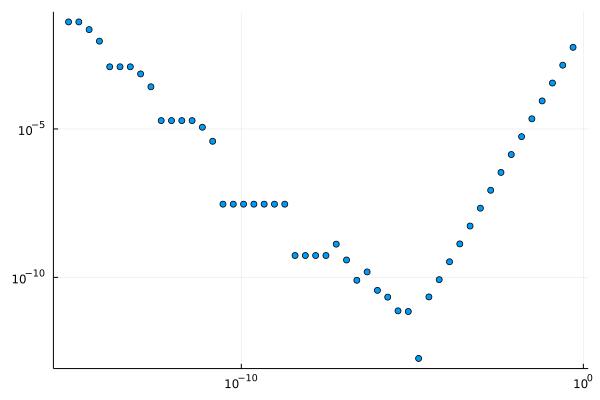
\includegraphics[width=10cm]{napaka_odvod.png}
    \caption{Napaka pri numeričnem računanju odvoda $\sin'(1)$}
    \label{fig:napaka_odvod}
\end{figure}


AD se izogne težavam zgornjih metod, zato mnogokrat predstavlja pomembno prednost in je prispevalo k pomembnem napredku različnih področij, kot so SU, Bayesova statistika, računalniški vid in mnogo drugih.

Pridevnik \textbf{avtomatičen} je velikokrat vir napačnega razumevanja koncepta AD in povzroča zamenjavo AD s simbolnim odvajanjem.
Pri AD ne gre za računanje analitičnega predpisov odvoda, pač pa za zaporedje numeričnih izračunov, ki vrnejo vrednost odvoda v neki točki. Prav tako ne gre za uporabo numeričnih aproksimacij odvoda kot pri numeričnem odvajanju, pač pa za numerično računanje odvoda v strojni natančnosti, pri kateri se vpliv zaokrožitvenih napak ne razlikuje bistveno od vpliva pri računanju same funkcije. Za razliko od ročne implementacije odvodov v kodi, AD zahteva le malo dodatnih vrstic v kodi, ki ne zahtevajo znanja pravil odvajanja ali lastnosti odvoda.

\begin{primer}
Pri analitičnem računanju odvoda produkta $h(x)=f(x)g(x)$
se pojavita tako $f(x)$ kot $f'(x)$. Če 
na koncu numerično ovrednotimo formulo za $h'(x)$, nekatera ovrednotenja skupnih faktorjev $f(x)$ in $f'(x)$ večkrat izvedemo. Temu pojavu rečemo \textbf{goltanje izrazov} in lahko proizvede simbolne izraze, katerih velikost narašča eksponentno s številom faktorjev v produktu.

Vzemimo
    $$f(x)=64x(1-x)(1-2x)^2(1-8x+8x^2)^2.$$
Potem je
    $$f'(x)=64(1-42x+504x^2-2640x^3+7040x^4-9984x^5+7168x^6-2048x^7).$$
Če bi računali numerično, bi lahko izkoristili pojavljanje izrazov $f_{1}(x)=x$, $f_{2}(x)=1-x$, $f_3(x)=1-2x$ in $f_4(x)=1-8x+8x^2$ v $f'(x)$.
Pišimo 
    $$g_i(x)=\big(\prod_{j\neq i}f_j(x)\big)\cdot f_3(x)f_4(x)$$ 
    za $i=1,2,3,4$. Potem je
    $$f'(x)=64g_{1}(x)-64g_{2}(x)-256g_3(x)f_3(x)+128g_4(x)\cdot(16x-8).$$
\end{primer}

\section{Avtomatsko odvajanje}

Na AD lahko gledamo kot na nestandardno interpretacijo računalniškega programa, pri čemer med izvajanjem programa računamo še vrednosti odvodov. Vse numerične operacije so kompozitumi končnega števila elementarnih funkcij, katerih odvode lahko izrazimo analitično. Kombiniranje teh odvodov z uporabo verižnega pravila nato numerično ovrednoti odvod oz.\ v primeru vektorske spremenljivke (oz.\ vektorske funkcije)  desni (oz.\ levi) smerni odvod. Med elementarne funkcije ponavadi štejemo spremembo predznaka, binarne aritmetične operacije in transcendentne funkcije (eksponentna, logaritemska in trigonometrijske funkcije).


\subsection{Računanje naprej}

Avtomatsko računanje odvoda naprej je konceptualno enostavnejši način AD. 
Začnemo tako, da za vsako vmesno spremenljivko $v_i$ 
izračunamo še njen odvod $\dot{v}_i=\frac{\partial v_i}{\partial x_j}$ po neodvisni spremenljivki $x_j$.
Z uporabo verižnega pravila za vsako spremenljivko med računanjem funkcijske vrednosti $F(a)$, $F:\RR^n\to \RR$, izračunamo še odvod. Na koncu računanja dobimo vrednost iskanega odvoda 
$\frac{\partial F(a)}{\partial x_j}$.

\subsubsection{Uporaba Wegnertovega seznama}
Ena od metod za naprejšnje računanja odvoda je s pomočjo \textbf{Wegnertovega seznama}.
Vpeljemo:
\begin{enumerate}
    \item \textbf{Vhodne spremenljivke:}
$v_{1-n}:=x_{1},\ldots,v_{0}:=x_n$.
    \item
\textbf{Delovne spremenljivke:}
    $v_{1},\ldots,v_\ell$. 
    \item 
\textbf{Izhodne spremenljivke:}
$y_{1}=v_{\ell-m+1}$, $y_{2}=v_{\ell-m+2}$,$\ldots$,$y_m=v_{\ell-m}$.
\end{enumerate}

Poglejmo si naprejšnji izračun na primeru.

\begin{primer}\label{260522-0821}
Dana je funkcija
    $$f(x_{1},x_{2})=\log(x_{1})+x_{1}x_{2}-\sin(x_{2}).$$ 
Zanimata nas vrednosti $f(2,5)$, ki jo označimo z $y$, in $\frac{\partial{f}}{\partial{x_{1}}}(2,5)$, z oznako $\dot{y}$.
V levi koloni bomo računali vrednosti funkcije, na desni pa vrednost odvoda, tako da vsako vrstico na levi strani odvajamo po $x_1$. Pri tem na začetku postavimo 
$\dot{v}_{-1}=\dot{x_1}=1$ in $\dot{v}_0=\dot{x_2}=0$.
\begin{align*}
    v_{-1}  &=x_{1}   
    =2,\quad
    &\dot{v}_{-1}
            =\dot{x}_{1}  =1,\\
    v_{0}     &= x_{2}  =5,\quad
    &\dot{v}_{0}= \dot{x}_{2} =0,\\
    v_{1}     &= \log(v_{-1})  =\log(2),\quad
    &\dot{v}_{1}= \frac{\dot{v}_{-1}}{v_{-1}}                =\frac{1}{2},\\
    v_{2}     &= v_{-1}v_{0}  =10,\quad
    &\dot{v}_{2}= \dot{v}_{-1} v_{0}+
                v_{-1}\dot{v}_{0} 
                =5+0=5,\\
    v_{3}     &= \sin(v_0)  =\sin(5),\quad
    &\dot{v}_{3}= \cos(v_0)\dot{v}_0 =0,\\
    v_{4}     &= v_1+v_2  =0.693+10,\quad
    &\dot{v}_{4}= \dot{v}_1+\dot{v}_2 =5.5,\\
    v_{5}     &= v_4-v_3  =10.693+0.959,\quad
    &\dot{v}_{5}= \dot{v}_{4}-\dot{v}_3 =5.5,\\
    y&=v_5=11.652,\quad 
    &\dot{y}=\dot{v}_5=5.5
\end{align*}

Drevo za izračun funckijske vrednosti $f(x_1,x_2)$ je naslednje:
\begin{center}
    \tikzstyle{every node}=[circle, draw, fill=black!0, inner sep=2pt, minimum width=5pt]
    \tikzset{edge/.style = {->,> = latex'}}
    
    \begin{tikzpicture}[thick,scale=1]%
        %nodes
        
        \node[draw] at (0,-1) (1) {$x_2$};
        \node[draw] at (2,-1) (2) {$v_0$};
        \node[draw] at (6,-1) (3) {$v_3$};
        \node[draw] at (4,1) (4) {$v_2$};
        \node[draw] at (8,1) (5) {$v_5$};
        \node[draw] at (10,1) (10)     {$f(x_1,x_2)$};
        \node[draw] at (0,3) (6) {$x_1$};
        \node[draw] at (2,3) (7) {$v_{-1}$};
        \node[draw] at (4,3) (8) {$v_1$};
        \node[draw] at (6,3) (9) {$v_4$};
        %edges
        
        \draw[edge] (1) -- (2);
        \draw[edge] (3) -- (5);
        \draw[edge] (5) -- (10);
        \draw[edge] (2) -- (4);
        \draw[edge] (4) -- (9);
        \draw[edge] (6) -- (7);
        \draw[edge] (7) -- (8);
        \draw[edge] (8) -- (9);
        \draw[edge] (7) -- (4);
        \draw[edge] (9) -- (5);
    \end{tikzpicture}
\end{center}
\end{primer}

Ta pristop se enostavno posploši na računanje Jacobijeve matrike. Če nas zanimajo odvodi po spremenljivki $x_i$,
na začetku postavimo $\dot{x}_i=1$ in $\dot{x}_j=0$ za $j\neq i$.
Tako lahko celotno Jacobijevo matriko
$$J_f=
\begin{pmatrix}
\frac{\partial y_1}{\partial x_1}&
\ldots &
\frac{\partial y_1}{\partial x_n}\\
\vdots & \ddots & \vdots\\
\frac{\partial y_m}{\partial x_1}&
\ldots &
\frac{\partial y_m}{\partial x_n}\\
\end{pmatrix}
$$
v $n$ korakih.
Hkrati lahko preprosto računamo smerni odvod $J_f\vec{r}$,
tako da na začetku postavimo $\dot{x}=\vec{r}$.
Torej lahko tudi to izračunamo samo v enem koraku naprej.

\subsubsection{Uporaba diferencialov}

\begin{primer}\label{260522-0920}
Dana je funkcija
    $$F(x_{1},x_{2})=e^{-x_1^2-x_2^2}.$$
Zanima nas vrednost smernega odvoda 
\begin{equation}\label{260522-0732}
\partial d_{\vec{v}}F(a_1,a_2)=
\begin{pmatrix}
\frac{\partial F(a_1,a_2)}{\partial x_1} &
\frac{\partial F(a_1,a_2}{\partial x_2}
\end{pmatrix}\vec{v}.
\end{equation}
Psevdokoda programa za avtomatičen izračun
smernega odvoda \eqref{260522-0732} je naslednja.

\begin{algorithm}[H]
\caption{Algoritem za izračun \eqref{260522-0732} }\label{alg:260522-0734}
\begin{algorithmic}\State
smerni\_odvod\_Gauss($x_1,x_2,v$)
\State\quad $a=x_1^2$
\State\quad $da=2*x_1*v(1)$
\State\quad $b=x_2^2$
\State\quad $db=2*x_2*v(2)$
\State\quad $c=a+b$
\State\quad $dc=da+db$
\State\quad $d=e^{-c}$
\State\quad $dd=-d*dc$
\State\quad return $d,dd$
\end{algorithmic}
 \end{algorithm}
Prepričajmo se o pravilnosti algoritma
\eqref{alg:260522-0734}.
Zapišimo sprva funkcijo $F$ kot kompozitium.
Ena od možnosti je naslednja:
\begin{equation}\label{260522-0928}
F(x_1,x_2)=(F_4\circ F_3\circ F_2\circ F_1)(x_1,x_2),
\end{equation}
kjer so
$$F_1(x_1,x_2)=(x_1^2,x_2),\quad
F_2(x_1,x_2)=(x_1,x_2^2),\quad
F_3(x_1,x_2)=-x_1-x_2,\quad
F_4(y)=e^{-y}.$$
Po verižnem pravilu velja
\begin{align}\label{260522-0929}
\begin{split}
(JF)(x)
&=
(JF_4)(F_3(F_2(F_1(x))))\cdot
(JF_3)(F_2(F_1(x)))\cdot
(JF_2)(F_1(x))\cdot
(JF_1)(x)\\
&=
-e^{-x_1^2-x_2^2}\cdot
\begin{pmatrix}
-1 & -1
\end{pmatrix}\cdot
\begin{pmatrix}
1 & 0\\
0 & 2x_2
\end{pmatrix}\cdot
\begin{pmatrix}
2x_1 & 0\\
0 & 1
\end{pmatrix}
\end{split}
\end{align}
Poglejmo si izračun smernega odvoda \eqref{260522-0732} po korakih, kar bo utemeljilo pravilnost izračuna v algoritmu 
\eqref{alg:260522-0734}.
\begin{align*}
((JF)(x))v
&=
\underbrace{-e^{-x_1^2-x_2^2}\cdot
\underbrace{\begin{pmatrix}
-1 & -1
\end{pmatrix}\cdot
\underbrace{\begin{pmatrix}
1 & 0\\
0 & 2x_2
\end{pmatrix}\cdot
\underbrace{\begin{pmatrix}
2x_1 & 0\\
0 & 1
\end{pmatrix}v}_{
(2x_1v_1, v_2)^T=(da,v_2)^T}}_{
(2x_1v_1, 2x_2v_2)^T=(da,db)^T
}}_{-2x_1v_1-2x_2v_2))=dc}}_{
-e^{-x_1^2-x_2^2}(-2x_1v_1-2x_2v_2)=dd}
\end{align*}
\end{primer}

\subsection{Dualna števila}

Odvajanje naprej lahko elegantno implementiramo z dualnimi števili.

\begin{definition}
Dualno število nad danim obsegom $\mathbb{O}$ je dvočlenik oblike 
$$a + b\varepsilon,$$
kjer sta števili $a$ in $b$ elementa obsega $\mathbb{O}$, $\varepsilon$ je dualna enota za katero velja $\varepsilon^2 = 0$.
\end{definition}

Pravila za računanje z \emph{dualnimi števili} so enaka kot pravila za računanje z dvočleniki, pri čemer moramo upoštevati, da je $\varepsilon ^2 = \varepsilon ^3 \ldots =0$. Tako je na primer produkt dveh dualnih števil enak

$$ (a +b\varepsilon)(c + d\varepsilon) = ac + (ad + bc)\varepsilon + bd\varepsilon^2 = ac + (ad + bc)\varepsilon.$$

Pri računanju z dualnimi števili lahko vse člene z višjimmi potencami $\varepsilon$ ignoriramo. Opazimo, da računska pravila za dualna števila sovpadajo s pravili za računanje z linearnim Taylorjevimi polinomi 

$$ T_1(f, x_0, x) = f(x_0) + f'(x_0)(x-x_0)$$

za funkcije okrog dane točke $x$, pri čemer $f(x_0)$ ustreza komponenti $a$, $f'(x_0)$ komponenti $b$, $(x-x_0)$ pa dualni enoti $\varepsilon$. Pravilo za produkt dveh funkcij je tako enako

$$T_1(f\cdot g, x_0, x) = f(x_0) + g(x_0) + \left(f'(x_0)g(x_0) + f(x_0)g'(x_0)\right)(x - x_0).$$

Zgornje pravilo lahko izpeljemo z dualnimi števili, če funkciji $f$ ozroma njeni linearni aproksimaciji v dani točki $x_0$ priredimo dualno število

$$d(f, x_0) = f(x_0) + f'(x_0)\varepsilon.$$

Pravila za računannje z dualnimi števili ustrezajo pravilom za odvajanje funkcij. Na primer vsota dualnih števil za dve funkije je enaka vsoti dualnega števila prirejenga vsoti funkcij

$$d(f, x_0) + d(g, x_0) = d(f + g, x_0)$$ 

Res 

$$(f(x_0) + f'(x_0)\varepsilon) + (g(x_0) + g'(x_0)\varepsilon) = f(x_0) + g(x_0) + (f'(x_0) + g'(x_0))\varepsilon.$$

Hitro lahko preverimo, da velja podobno za vse osnovne računske operacije 
\begin{eqnarray*}
d(f, x_0)d(g, x_0) &=& d(fg, x_0)\\
d(f, x_0)/d(g, x_0) &=& d(f/g, x_0)\\
d(f, x_0)^n & =& d(f^n, x_0)\\
...
\end{eqnarray*} 

Na primer, pravilo za odvod kvocienta lahko dobimo z deljenjem dualnih števil:

\begin{multline*}
    \frac{f(x_0) + f'(x_0)\varepsilon}{g(x_0) + g'(x_0)\varepsilon} = \frac{(f(x_0) + f'(x_0)\varepsilon)(g(x_0) - g'(x_0)\varepsilon)}{(g(x_0) + g'(x_0)\varepsilon)(g(x_0) - g'(x_0)\varepsilon)} = \frac{f(x_0)}{g(x_0)} + \frac{f'(x_0)g(x_0) - f(x_0)g'(x_0)}{g(x_0)^2}\varepsilon.
\end{multline*}

\begin{theorem}
Aritmetika dualnih števil popolnoma ustreza aritmetiki linearnih aproksimacij funkcije v dani točki.
\end{theorem}


\subsubsection{Dualna števila za funkcije več spremenljivk}

$$d(f, \vec{x}) = f(\vec{x}) + \frac{\partial f}{\partial x_1}(\vec{x})\varepsilon_1 + \frac{\partial f}{\partial x_2}(\vec{x})\varepsilon_2\ldots \frac{\partial f}{\partial x_n}(\vec{x})\varepsilon_n  $$

pri čemer velja $\varepsilon_i\varepsilon_j = 0$.

\subsubsection{Implementacija AD z dualnimi števili}

dualna števila lahko preprosto uporabimo za implementacijo avtomatskega odvajanja v jezikih, ki podpirajo polimorfizem operatorjev in funkcij. Definirati moramo nov razred ali podatkovni tip, ki poleg vrednosti hrani še 
vrednost odvoda in implementirati aritmetiko dualnih števil za ta podatkovni tip. Na ta način lahko odvajamo vse generične funkcije implementirane v danem programskem jeziku. Generične funkcije za argumente ne zahtevajo točno določenega podatkovnega tipa, ampak dopuščajo poljubne podatkovne tipe, ki podpirajo operacije, ki so uporabljene znotraj funkcije. Odvod generične fukcije dobimo tako, da namesto števila, kot parameter vstavimo dualno število.

Poglejmo si primer v Pythonu za računanja kvadratnega korena z babilonskim obrazcem.

\subsubsection{Dualna števila za višje odvode}

$$d_n(f, x) = f(x) + f'(x)\varepsilon_1 + \frac{f''(x)}{2}\varepsilon_2\ldots \frac{f^{(n)}(x)}{n!}\varepsilon_n,$$

pri čemer velja $\varepsilon_i\varepsilon_j = \varepsilon_{i+j}$ in $\varepsilon_k = 0$ za $k>n$.


S kombinacijo dualnih števil za funkcije več spremenljivk in višjih odvodov, lahko implementiramo AD, ki omogoča računanje odvodov do določene stopnje.

\subsection{Vzvratno računanje}

AD z vzvratnim računanjem računa odvode v obratni smeri. Za vsako vmesno spremenljivko $v_i$ izračunamo še njeno pomožno spremenljivko $\bar v_i=\frac{\partial G_j}{\partial v_i}$, kjer je $G=(G_1,\ldots,G_p):\RR^m\to \RR^p$. Kot rezultat bomo dobili vrednost 
$\frac{\partial G_j(b)}{\partial x_j}$,
kjer je $b\in \RR^m$.

Pri vzvratnem računanju odvode računamo na drugi stopnji dvostopenjskega postopka. Na prvi stopnji izračunamo funkcijske vrednosti s pomočjo Wegnertovega seznama, na drugi stopnji pa izračunamo odvode prek računanja 
vrednosti pomožnih spremenljivk $\bar v_i$ v vzvratni smeri.

Poglejmo si vzvratni izračun na primeru \ref{260522-0821}.

\begin{primer}
Naj bo $f(x_1,x_2)$ funkcija kot v primeru \ref{260522-0821}.
Zanimata nas vrednosti $\frac{\partial f}{\partial x_1}(2,5)$, $\frac{\partial f}{\partial x_2}(2,5)$.
Kot v primeru \ref{260522-0821} označimo $y=f(2,5)$. Tako želimo izračunati $\frac{\partial{y}}{\partial x_1}=\bar x_1$ in
$\frac{\partial{y}}{\partial x_2}=\bar x_2$ 
oz.\ s pomočjo spremenljivk $v_i$, 
V levi koloni sprva izračunamo vrednosti funkcije, potem pa računamo desno kolono od spodaj navzgor. Pri tem na začetku postavimo 
$\bar{y}=\frac{\partial y}{\partial y}=1$
\begin{align*}
    v_{-1}  &=x_{1}   
    =2,\quad
    &\bar{x}_1=\bar{v}_{-1}=5.5,\\
    v_{0}     &= x_{2}  =5,\quad
    &\bar x_2=\bar{v}_{0}=1.716,\\
    v_{1}     &= \log(v_{-1})  =\log(2),\quad
    &\bar{v}_{-1}=
        \bar{v}_{-1}+
        \bar{v_1}
        \frac{\partial v_1}{\partial v_{-1}}=
        \bar{v}_{-1}+
        \bar{v_1}
        \frac{1}{v_{-1}}              =5.5,\\
    v_{2}     &= v_{-1}v_{0}  =10,\quad
    &\bar{v}_{-1}= \bar{v}_{2} 
        \frac{\partial v_2}{\partial v_{-1}}
        =\bar v_2 v_0=5,\\
    &\quad
    &\bar{v}_{0}=  \bar v_0+\bar{v}_{2} 
        \frac{\partial v_2}{\partial v_{0}}
        =\bar v_0+\bar v_2 v_{-1}=1.716,\\
    v_{3}     &= \sin(v_0)  =\sin(5),\quad
    &\bar{v}_{0}= \bar v_3\frac{\partial v_3}{\partial v_0} =\bar v_3 \cos(v_0)=-0.284,\\
    v_{4}     &= v_1+v_2  =0.693+10,\quad
    &\bar{v}_{1}= \bar{v}_4\frac{\partial v_4}{\partial v_1}=\bar v_4=1,\\
    &\quad 
    &\bar{v}_{2}= \bar v_4
    \frac{\partial v_4}{\partial v_2}=\bar v_4=1,\\
    v_{5}     &= v_4-v_3  =10.693+0.959,\quad
    &\bar{v}_{3}= \bar v_5
    \frac{\partial v_5}{\partial v_3}=-\bar v_5=-1,\\
    &\quad 
    &\bar{v}_{4}= \bar v_5
    \frac{\partial v_5}{\partial v_4}=\bar v_5=1,\\
    y&=v_5=11.652,\quad 
    &\bar{y}=\bar{v}_5=1
\end{align*}
V drevesu funkcije $f$ (glej primer \ref{260522-0821}) vidimo, da na spremembo $y$ spremenljivka $v_{-1}$ vpliva preks spremenljivk $v_2$ in $v_1$. Torej njen prispevek izračunamo kot
$$\frac{\partial y}{\partial v_{-1}}=
\frac{\partial y}{\partial v_2}
\frac{\partial v_2}{\partial v_{-1}}
+
\frac{\partial y}{\partial v_1}
\frac{\partial v_1}{\partial v_{-1}}
\quad\text{oziroma}\quad
\bar v_{-1}
=
\bar v_2
\frac{\partial v_2}{\partial v_{-1}}
+
\bar v_1
\frac{\partial v_1}{\partial v_{-1}}
$$
\end{primer}

\subsubsection{Uporaba diferencialov}

\begin{primer}
Dana je funkcija $F(x_1,x_2)$
kot v primeru \eqref{260522-0920}.
Zanima nas gradient
\begin{equation}\label{260522-0921}
\nabla F(a_1,a_2)=
\begin{pmatrix}
\frac{\partial F(a_1,a_2)}{\partial x_1} &
\frac{\partial F(a_1,a_2)}{\partial x_2}
\end{pmatrix}.
\end{equation}
Psevdokoda programa za avtomatičen izračun
gradienta \eqref{260522-0921} je naslednja.

\begin{algorithm}[H]
\caption{Algoritem za izračun \eqref{260522-0921} }\label{alg:260522-0921}
\begin{algorithmic}\State
gradient\_Gauss($x_1,x_2$)
\State\quad $a=x_1^2$
\State\quad $da=2*x_1$
\State\quad $b=x_2^2$
\State\quad $db=2*x_2$
\State\quad $c=a+b$
\State\quad $dc=\left[\begin{array}{cc} 1 & 1\end{array}\right]$
\State\quad $d=e^{-c}$
\State\quad $dd=-d$
\State\quad $\grad=1$
\State\quad $\grad=dd$
\State\quad $\grad=\grad*dc$
\State\quad $\grad(2)=\grad(2)*db$
\State\quad $\grad(1)=\grad(1)*da$
\State return $\grad$
\end{algorithmic}
\end{algorithm}
Prepričajmo se o pravilnosti algoritma
\eqref{alg:260522-0921}.
Naj bo $F$ zapisan kot kompozitium
\eqref{260522-0928} in 
$JF$ njegova Jacobijeva matrika kot v \eqref{260522-0929}.
Poglejmo si izračun gradienta \eqref{260522-0921} po korakih, kar bo utemeljilo pravilnost izračuna v algoritmu 
\ref{alg:260522-0921}.
\begin{align*}
(JF)(a)
&=
\underbrace{\underbrace{\underbrace{\underbrace{-e^{-x_1^2-x_2^2}}_{dd}\cdot
\begin{pmatrix}
-1 & -1
\end{pmatrix}}_{(dd,dd)}
\cdot 
\begin{pmatrix}
1 & 0\\
0 & 2x_2
\end{pmatrix}}_{(dd,dd\cdot db)}\cdot
\begin{pmatrix}
2x_1 & 0\\
0 & 1
\end{pmatrix}}_{(dd\cdot da,dd\cdot db)}
\end{align*}
\end{primer}

\section{Odvisnost rešitve NDE od parametrov}

Poglejmo si primer, ko želimo analizirati, kako je rešitev začetnega problema za navadne diferencialne enačbe (NDE) odvisna od parametrov. Navadne difrencialne enačbe, večinoma nimajo analitičnih rešitev. V praksi rešitev poiščemo numerično.
Če v enačbi nastopjo parametri, je odvisnost rešitve začetnega problema od parametrtov podana implicitno. Simbolno računanje odvoda, tako ne pride v poštev.
Numerično odvajanje pomeni večkratno numerično reševanje začetnega problema, kar je časovno lahko zelo zahtevno.  

\begin{thebibliography}{1}

\bibitem{}

\end{thebibliography}
\end{document}